\section{Introduction}
\label{sec:Introduction}

The \lhcb experiment uses two ring-imaging Cherenkov (\rich) detectors to provide powerful discrimination between charged particles in the intense hadron production environment of the \lhc. These two separate \rich detectors have different radiators and are designed to provide particle identification over a momentum range of 1 to $100\gevc$~\cite{Alves:2008zz}. The performance of the particle identification supplied by the \rich system~\cite{LHCb-DP-2012-003} strongly depends on the quality of its alignment, i.e. how accurately the physical position of each component of the \rich detectors is described in the \lhcb software. The goal of the alignment procedure is determine the exact position of all optical components and propagate this information to the \lhcb conditions database that stores the non-event time-varying data pertaining to detector conditions.\\
The \lhcb detector achieved excellent performance in Run I but faces more challenging conditions in Run II. The \lhc will collide protons at an increased centre-of-mass energy of 13\tev and with 25\ns bunch spacing. The spatial alignment of the detector and the accurate calibration of its subcomponents are essential to achieve the best physics performance. In order to keep the selection efficiencies in the high level trigger as high as in Run I, conditions on the particle identification will be used in Run II. This requires the full alignment and calibration of the \rich detectors within the high performance trigger sequence.\\
This note describes how the \lhcb \rich optical systems are aligned in software in Run II using proton-proton collision data. The method used is discussed in
\sect{sec:MirrorAlignmentMethod}, while the computing framework and the implementation for the automated running of the alignment is described in \sect{sec:OnlineAlignmentFramework}. The results for the data-taking period in 2015 are presented in Section \ref{XXX}.\\

\begin{equation}
O = \frac{\sum^{ADC>thresh.}N_{events}}{\sum N_{events}}
\end{equation}

\section{The \lhcb detector}

The \lhcb detector~\cite{Alves:2008zz, LHCb-DP-2014-002} is a single-arm forward spectrometer covering the \mbox{pseudorapidity} range $2<\eta <5$, designed for the study of particles containing \bquark or \cquark quarks. The detector includes a high-precision tracking system consisting of a silicon-strip vertex detector surrounding the $pp$ interaction region, a large-area silicon-strip detector located upstream of a dipole magnet with a bending power of about $4{\mathrm{\,Tm}}$, and three stations of silicon-strip detectors and straw drift tubes placed downstream of the magnet. The tracking system provides a measurement of momentum, \ptot, of charged particles with
a relative uncertainty that varies from 0.5\% at low momentum to 1.0\% at 200\gevc. The minimum distance of a track to a primary vertex, the impact parameter, is measured with a resolution of $(15+29/\pt)\mum$, where \pt is the component of the momentum transverse to the beam, in\,\gevc. \\
Different types of charged hadrons are distinguished using information from two ring-imaging Cherenkov detectors~\cite{LHCb-DP-2012-003}. Photons, electrons and hadrons are identified by a calorimeter system consisting of scintillating-pad and preshower detectors, an electromagnetic calorimeter and a hadronic calorimeter. Muons are identified by a system composed of alternating layers of iron and multiwire proportional chambers.\\
The event selection is performed by a trigger, which consists of a hardware stage, based on information from the calorimeter and muon systems, followed by a software stage, which applies a full event reconstruction.\\
In Run II, the alignment and calibration of all subdetectors is performed online in between different stages of the high level trigger (\hlt) and the results are immediately applied to the reconstruction.


\subsection {\rich optical systems}

Both \richone and \richtwo have two sets of mirrors: the primary spherical mirrors, and the secondary (a.k.a. plane, flat), much flatter mirrors. Cherenkov photons emitted by a charged track are reflected off a primary mirror onto a secondary mirror, and from there out of the \lhcb acceptance onto the plane of photon detectors, which coincides with the focal plane of the given part of the optical systems. The \richone/\richtwo optical systems consists of 4/56 primary and 16/40 secondary mirrors. The layouts of the \rich optical systems are shown in Figure \ref{fig:RICH_OpticalLayout} \cite{LHCB:2000aa,LHCb:2003ab}, while the structures of the mirror arrays and their numbering are shown in Figures \ref{fig:RICH1_MirrorNumbering} and~\ref{fig:RICH2_MirrorNumbering} of Section \ref{sec:MirrorAlignmentMethod}.

\begin{figure}[h!]
  \vspace{-0.5\baselineskip}
  \centering{
    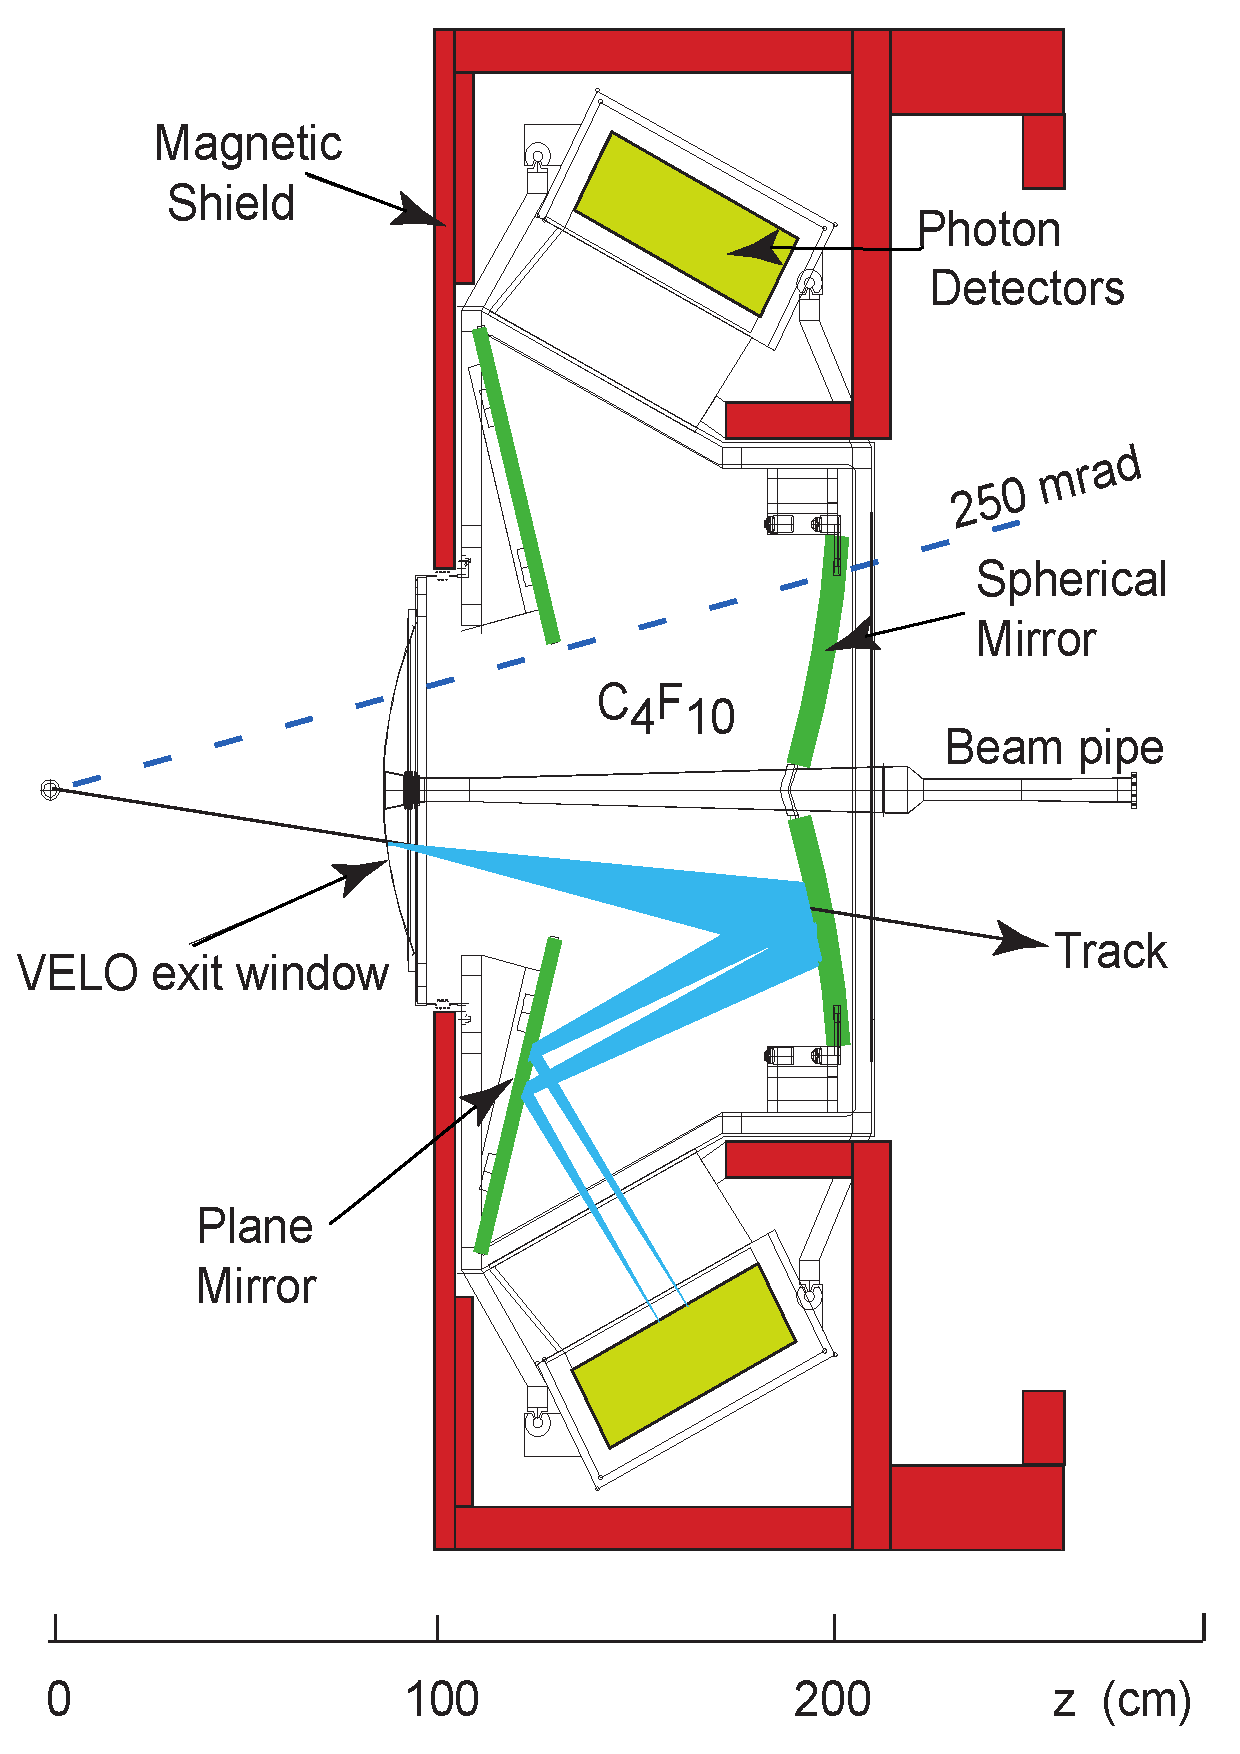
\includegraphics[width=0.49\textwidth,trim={0.0cm -0.45cm 0.0cm 0.0cm}]{figs/Introduction/rich1-2d-schematic.pdf}
    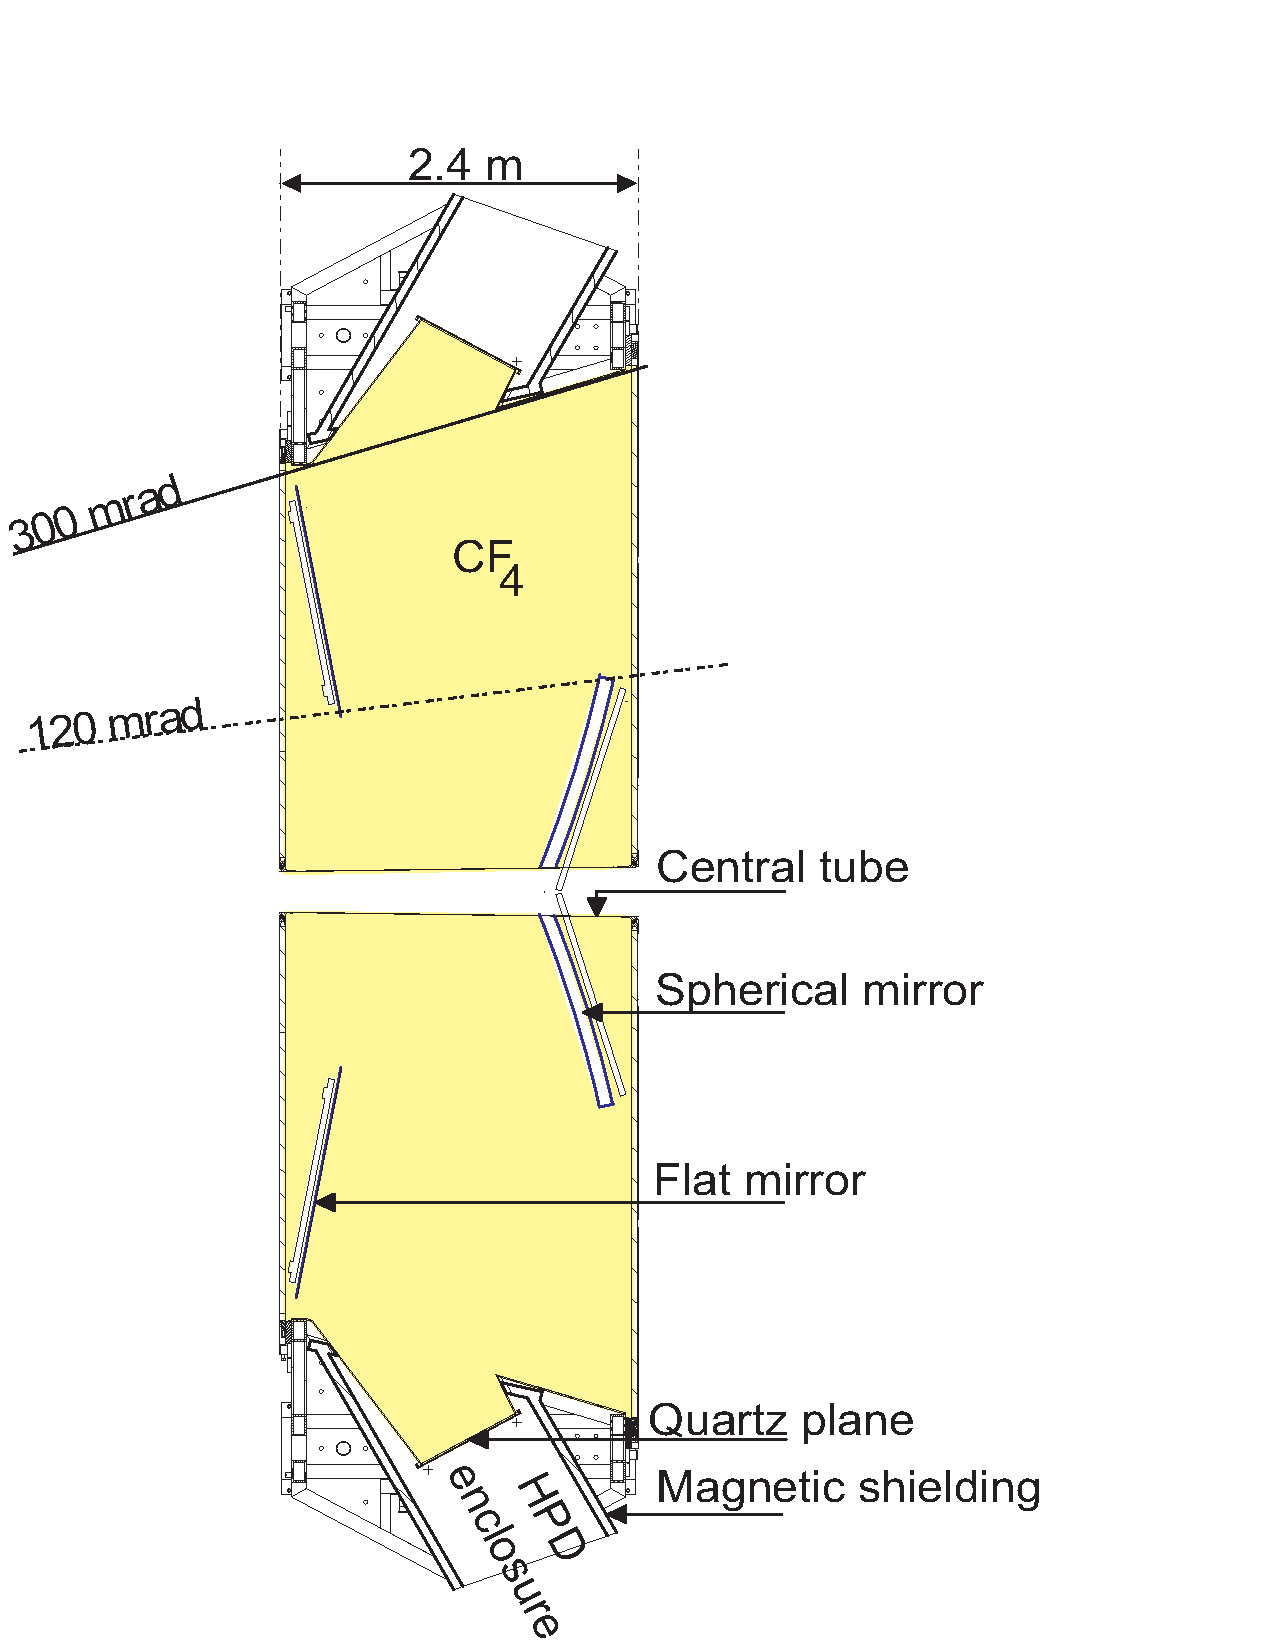
\includegraphics[width=0.49\textwidth,trim={0.0cm  0.0cm  3.5cm 2.5cm}]{figs/Introduction/RICH2_2d.pdf}
  }
  \hspace{0.51\textwidth}(a)\hspace{0.47\textwidth}(b)\hspace{0.02\textwidth}
  \vspace{-0.5\baselineskip}
  \caption{
    Schematic view of the LHCb RICH detectors and their optical systems:
    (a) side view of \richone and (b) top view of \richtwo. Formation of a
    Cherenkov ring in the lower part of \richone is also drawn.}
  \label{fig:RICH_OpticalLayout}
  \vspace{-0.5\baselineskip}
\end{figure}


The right-handed coordinate system of each mirror segment is defined by placing the origin at the centre of curvature with the $x$-axis pointing towards the mirror, the $y$-axis pointing upwards and the corresponding $z$-axis being horizontal. Finally, the pivot point for the software rotations around the $y$- and $z$-axes is at the centre of each mirror.\\
In order to achieve the optimal performance of the \lhcb \rich detector we aim to minimize the uncertainty, $\sigma$, associated with the measurement of a single photon Cherenkov angle. This is limited by four main sources of uncertainty outlined in Table \ref{tab:RichErrors}. Adding them in quadrature gives the minimal total uncertainty, which can be obtained by having an optimal alignment of all optical components of the \rich detectors.
\begin{table}[htb]
  \vspace{-0.5\baselineskip}
  \caption{
    Sources of uncertainty, $\sigma$, of the measurement of a single photon
    Cherenkov angle for the three \lhcb RICH radiators.}
  \vspace{-0.5\baselineskip}
  \centering
  \begin{tabular}{lcc}
                           &\multicolumn{2}{c}{$\sigma\,[\mathrm{mrad}]$}  \\
    \cmidrule(r){2-3}
                           &\richone&\richtwo  \\
    \cmidrule(r){2-3}
                            &   $\cfourften$   & $\cffour$\\
    \midrule
    \midrule
      Emission point        &      0.8         &     0.2  \\
      Chromatic dispersion   &      0.9         &     0.5  \\
      Pixel size            &      0.6         &     0.2  \\
      Tracking                &      0.4         &     0.4  \\
      \hline
      Total                &      1.5         &     0.7  \\
  \end{tabular}
  \label{tab:RichErrors}
  \vspace{-0.5\baselineskip}
\end{table}
